\documentclass[pscyr]{hedlab}
\usepackage[russian]{babel}
\usepackage{graphicx}
\graphicspath{{images/}}
\usepackage{listings}

\lstset{
    basicstyle=\footnotesize,
    inputencoding=utf8,
    extendedchars=True,
    language=[Sharp]C,
    numbers=left,
    numberstyle=\footnotesize,
    breakatwhitespace=\false,
    breaklines=True,
    tabsize=2,
    keepspaces=true,
}

\labname{Создание Web-служб}
\labnum{7}
\student{Голубев~А.~В., САПР-1.1п}
\labdate{}

\begin{document}
    \makeheader
    \emph{Цель:} получение практических навыков создания веб-служб и реализации вызов веб-методов 
    из ASP.NET приложения.\\
    \emph{Задачи:} 
    \begin{enumerate}
        \item Создать веб-службу, реализующую несколько веб-методов.
        \item Реализовать вызов методов веб-сервиса в ASP.NET приложении.
    \end{enumerate}
    Исходный код Web-службы:
    \lstinputlisting{./code/service.cs}
    Вызов функций Web-службы:
    \lstinputlisting{./code/page.cs}
    Хранимые процедуры:
    \lstinputlisting[inputencoding=utf8,basicstyle=\footnotesize,language=SQL]{./code/lab07.sql}

    \pagebreak

    \begin{figure}[h!]
        \center
        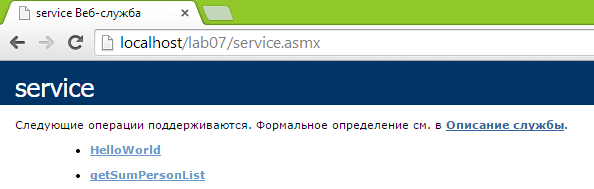
\includegraphics[width=.60\textwidth]{lab07_02} \\
        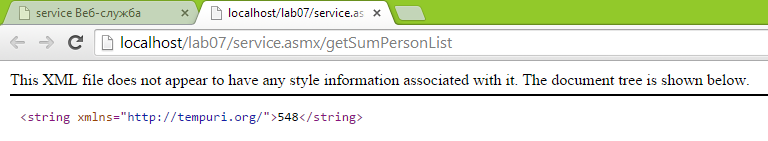
\includegraphics[width=.60\textwidth]{lab07_03} \\
        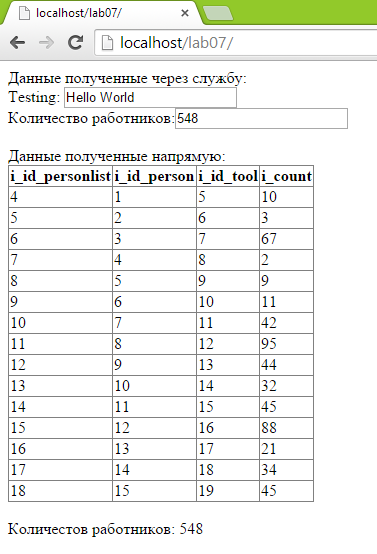
\includegraphics[width=.47\textwidth]{lab07_01}
    \end{figure}

    \emph{Вывод:} в результате проделанной работы
    \begin{enumerate}
        \item Создал веб-службу, реализующую несколько веб-метода.
        \item Реализовал вызов методов веб-сервиса в ASP.NET приложении.
    \end{enumerate}
\end{document}